\documentclass{beamer}
\usetheme{Goettingen}
\usecolortheme{seahorse}
\usepackage[ruled,linesnumbered]{algorithm2e}
\usepackage{graphicx}
\usepackage[absolute,overlay]{textpos}
\title{Chapter 6 Linear Model Selection and Regularization}
\author{Zhenmiao Zhang}
\setbeamertemplate{footline}[frame number]
\setbeamercolor{footline}{fg=beamer@blendedblue}
\setbeamerfont{section in sidebar}{size=\fontsize{5.5}{6}\selectfont}
\setbeamerfont{subsection in sidebar}{size=\fontsize{5}{5.5}\selectfont}
\begin{document}

	\begin{frame}
	    \maketitle
	\end{frame}
	
	\section{Overview}
	
	\begin{frame}{Outline}
		\tableofcontents
	\end{frame}

	\subsection{Motivation}
	
	\begin{frame}{Linear Regression}
		The standard linear regression model with $p$ predictors:
		\[
		Y=\beta_0 + \beta_1X_1+ ... + \beta_pX_p + \epsilon .
		\]
		The model is typically fit with least squares. For $n$ observations:
		\begin{align*}
			&X=[x_1, x_2, ..., x_n]^T \in \mathbb{R}^{n\times (p+1)}, \\
			&Y=[y_1, y_2, ..., y_n]^T \in \mathbb{R}^{n\times 1}, \\
			&\beta=[\beta_0, \beta_1, ..., \beta_p]^T \in \mathbb{R}^{(p+1)\times 1},
		\end{align*}
		the estimated $\hat{\beta}$ should be:
		\begin{align*}
			&\hat{\beta} = \mathop{\arg\min}_{\beta} \|Y-X\beta\|_2^2 \Rightarrow \frac{\partial \|Y-X\beta\|_2^2}{\partial \beta}=0 \\
			&\Rightarrow -X^T(Y-X\hat{\beta})=0 \Rightarrow \hat{\beta}=(X^TX)^{-1}X^TY.
		\end{align*}
	\end{frame}

	\begin{frame}{Number of observations and predictors}
		Number of observations: $n$\\
		Number of predictors: $p$ ($p+1$ coefficients)
		\begin{itemize}
			\item $p \ll n$: the least squares estimates tend to have low variance, and will perform well on test observations.
			\item $p\approx n$: there can be high variability in the least squares fit, resulting in overfitting and consequently poor predictions on test set.
			\item $p \geq n$: there is no longer a unique least squares coefficient estimate; the variance is infinite; the MSE on an independent test set becomes extremely large.
		\end{itemize}
		\textbf{We need exclude irrelevant variables from a multiple regression model!}
	\end{frame}
	
	\section{Subset Selection}
	
	\begin{frame}{Outline}
		\tableofcontents[currentsection]
	\end{frame}

	\subsection{Best Subset Selection}
	
	\begin{frame}{Best Subset Selection}
		Best Subset Selection: fit a separate least squares regression for each possible combination of the $p$ predictors; select the best model from among the $2^p$ possibilities.
		\begin{algorithm}[H]
			\caption{Best Sample Selection}
			Let $M_0$ denote the null model with no predictors. It simply predicts the sample mean for each observation. \\
			\For{$k = 1, 2, . . . p$}{
				Fit all $\binom{p}{k}$ models that contain exactly $k$ predictors.\\
				Pick the best among these $\binom{p}{k}$ models, and call it $M_k$. Here best is defined as having the smallest $RSS$, or equivalently largest $R^2$.
			}
			Select a single best model from among $M_0, . . . , M_p$ using cross-validated prediction error, $C_p (AIC), BIC$, or adjusted $R^2$.
		\end{algorithm}
	\end{frame}
	
	\begin{frame}{How to select the best model?}
		\textbf{Indirect approach}: we can estimate test error by making an adjustment to the training error:
		\begin{itemize}
			\item $C_p$ estimate of test MSE: $C_p = \dfrac{1}{n}(RSS+2d\hat{\sigma}^2)$
			\item $AIC$ for maximum likelihood: $SIC=\dfrac{1}{n\hat{\sigma}^2}(RSS+2d\hat{\sigma}^2)$
			\item $BIC$ from Bayesian: $BIC=\dfrac{1}{n\hat{\sigma}^2}(RSS+log(n)d\hat{\sigma}^2)$
			\item Adjusted $R^2$: Adjusted $R^2 = 1-\dfrac{RSS/(n-d-1)}{TSS/(n-1)}$
		\end{itemize}
		\textbf{Direct approach}: we can directly estimate the test error, using either a validation set or a cross-validation method.
	\end{frame}
	
	\begin{frame}{Indirect approach}
		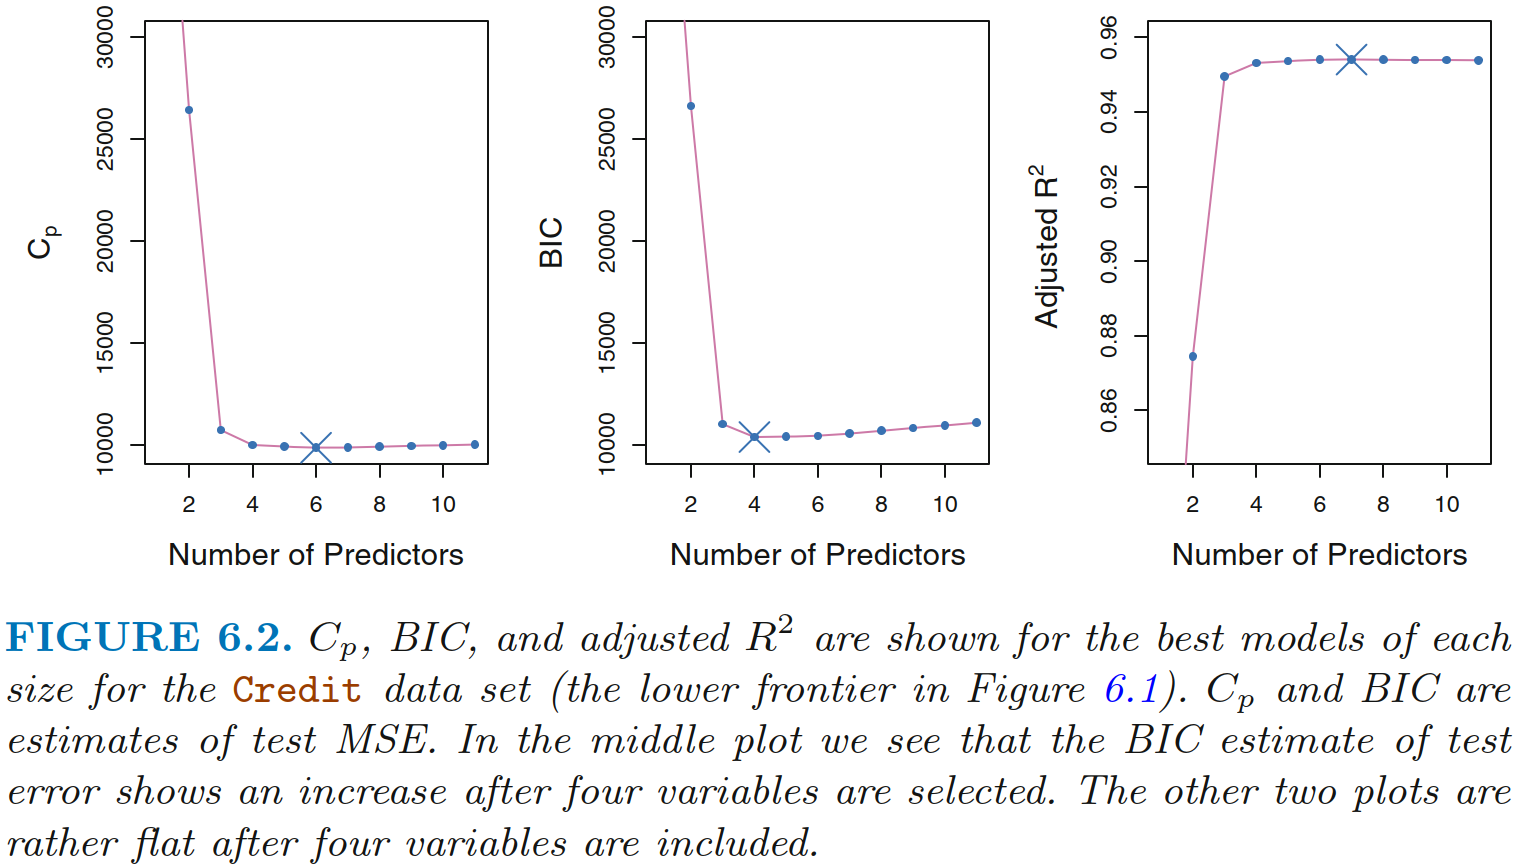
\includegraphics[width=10cm]{figure_6.2.png}
	\end{frame}
	
	\begin{frame}{Direct approach}
		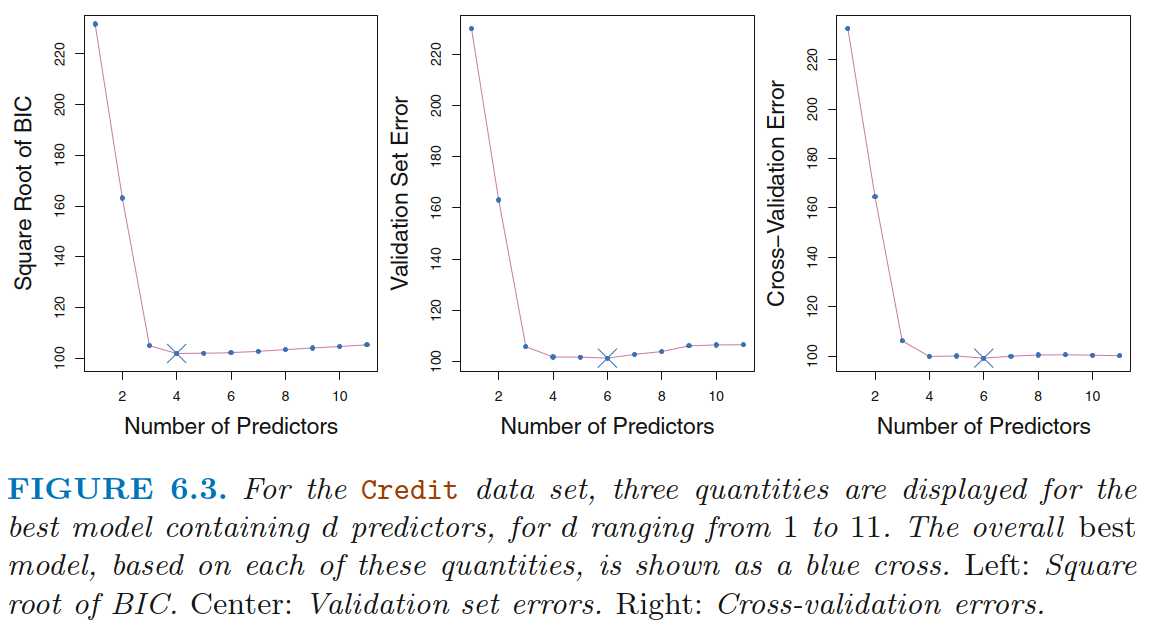
\includegraphics[width=10cm]{figure_6.3.png}
	\end{frame}
	
	\begin{frame}{Drawbacks of best subset selection}
		Best subset selection has two main drawbacks:
		\begin{itemize}
			\item For computational reasons, best subset selection cannot be applied with very large $p$ ($p \geq 40$).
			\item An enormous search space can lead to overfitting and high variance of the coefficient estimates. \textbf{Guided search} is necessary.
		\end{itemize}
	\end{frame}

	\subsection{Stepwise Selection}
	\begin{frame}{Forward Stepwise Selection}
		Alternative - Forward Stepwise Selection: select the best model only from $1+p(p+1)/2$ models.
		\begin{algorithm}[H]
			\caption{Forward Stepwise Selection}
			Let $M_0$ denote the null model with no predictors. \\
			\For{$k = 0, 1, . . . p-1$}{
				Consider all $p-k$ models that augment the predictors in $M_k$ with one additional predictor.\\
				Choose the best among these $p-k$ models, and call it $M_{k+1}$. The best is defined as having smallest $RSS$, or largest $R^2$.
			}
			Select a single best model from among $M_0, . . . , M_p$ using cross-validated prediction error, $C_p (AIC), BIC$, or adjusted $R^2$.
		\end{algorithm}
	\end{frame}

	\begin{frame}{Backward Stepwise Selection}
		Alternative - Backward Stepwise Selection: begins with the full least squares model.
		\begin{algorithm}[H]
			\caption{Backward Stepwise Selection}
			Let $M_p$ denote the full model, which contains all $p$ predictors. \\
			\For{$k = p, p-1, . . . 1$}{
				Consider all $k$ models that that contain all but one of the predictors in $M_k$, for a total of k − 1 predictors.\\
				Choose the best among these $k$ models, and call it $M_{k-1}$. The best is defined as having smallest $RSS$, or largest $R^2$.
			}
			Select a single best model from among $M_0, . . . , M_p$ using cross-validated prediction error, $C_p (AIC), BIC$, or adjusted $R^2$.
		\end{algorithm}
	\end{frame}
	
	\begin{frame}{Hybrid Approach}
		\begin{itemize}
			\item Similarly to forward selection, variables are added to the model sequentially.
			\item After adding each new variable, the method may also remove any variables that no longer provide an improvement in the model fit.
			\item Better model space exploration while retaining computational advantages of both stepwise selections.
		\end{itemize}
	\end{frame}

	\begin{frame}{Comparison of the stepwise selection approaches}
		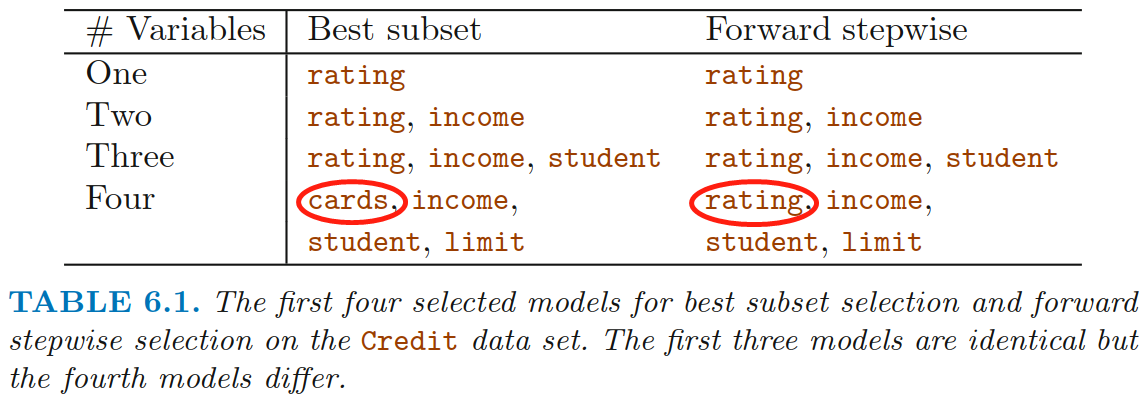
\includegraphics[width=10cm]{table_6.1.png}
		\begin{itemize}
			\item Forward stepwise, backward stepwise and hybrid approach are not guaranteed to yield the best model containing a subset of the $p$ predictors.
			\item Forward stepwise and hybrid approach can be used even when $n \leq p$. In this case, it is possible to construct sub-models $M_0, ..., M_{n-1}$ only.
		\end{itemize}
	\end{frame}
	
	\section{Shrinkage Methods}
	\begin{frame}{Outline}
		\tableofcontents[currentsection]
	\end{frame}

	\subsection{Ridge Regression}
	\begin{frame}{Ridge Regression}
		\[
		\hat{\beta}^R = \mathop{\arg\min}_{\beta} \sum_{i=1}^{n} (y_i-\beta_0-\sum_{j=1}^{p} \beta_jx_{ij})^2+\lambda\sum_{j=1}^{p}\beta_j^2
		\]
	\end{frame}
	
	\begin{frame}{Centered trick for bias term}
		Transform the training data to centered form:
		\begin{align*}
			&X=[x_1-\overline{x},...,x_n-\overline{x}]^T \\
			&Y=[y_1-\overline{y}, ..., y_n-\overline{y}]^T \\
			&\beta=[\beta_1, ..., \beta_p]^T, \beta_0=\overline{y}-\beta^T\overline{x}
		\end{align*}
		Ridge Regression (centered):
		\begin{equation}
			\hat{\beta}^R = \mathop{\arg\min}_{\beta} \|X\beta-Y\|_2^2 + \lambda \|\beta\|_2^2
		\end{equation}
		Another formulation (centered):
		\begin{equation}
			\hat{\beta}^R = \mathop{\arg\min}_{\beta} \|X\beta-Y\|_2^2,\ s.t.\ \|\beta\|_2^2 \leq s
		\end{equation}
	\end{frame}
	
	\begin{frame}{Proof of equivalence}
		\textit{Proof} \\
		Both (1) and (2) are convex programming, thus the K-K-T are sufficient and necessary conditions to optimal points. \\
		The Lagrange function of (2):
		\[
		L_2(\beta;\lambda_{L_2})=\|X\beta-Y\|_2^2+\lambda_{L_2}(\|\beta\|_2^2-s).
		\]
		K-K-T conditions:
		\begin{align*}
			&\frac{\partial L_2(\beta;\lambda_{L_2})}{\partial \beta}=0, \\
			&\|\beta\|_2^2-s \leq 0, \\
			&\lambda_{L_2} \geq 0, \\
			&\lambda_{L_2}(\|\beta\|_2^2-s)=0.
		\end{align*}
	\end{frame}
	
	\begin{frame}{Proof of equivalence}
		The Lagrange function of (1):
		\[
		L_1(\beta)=\|X\beta-Y\|_2^2+\lambda\|\beta\|_2^2.
		\]
		K-K-T conditions:
		\begin{align*}
			&\frac{\partial L_1(\beta)}{\partial \beta}=0. \\
		\end{align*}
		Let $\lambda_{L_2}=\lambda \geq 0$, we have $\frac{\partial L_2(\beta;\lambda_{L_2})}{\partial \beta} = \frac{\partial L_1(\beta)}{\partial \beta}$. \\
		Considering K-K-T are sufficient and necessary conditions, all the optimal points of (1) are optimal points of (2), and vice versa (let $s=\|\hat{\beta}\|_2^2$ when $\lambda\ne0$).
		\begin{proof}[\unskip\nopunct]\end{proof}
	\end{frame}

	\begin{frame}{Solution of ridge regression}
		From the K-K-T conditions of (1), we can directly give the estimate of $\beta$:
		\begin{align*}
			&\frac{\partial L_1(\beta)}{\partial \beta}=0 \Rightarrow X^T(X\hat{\beta}^R-Y)+\lambda \hat{\beta}^R=0 \\
			&\Rightarrow \hat{\beta}^R=(X^TX+\lambda I)^{-1}X^TY
		\end{align*}
		If $\lambda \ne 0$, we have $s=\|\hat{\beta}^R\|_2^2=\|(X^TX+\lambda I)^{-1}X^TY\|_2^2$. \\
		If $\lambda=0$, $\hat{\beta}^R=(X^TX)^{-1}X^TY=\hat{\beta}$ (least square).
	\end{frame}
	
	\begin{frame}{Bayesian interpretation of ridge regression}
		Ridge regression is maximum a posteriori estimation (MAP) that assumes $\beta$ has prior distribution of $\beta \sim \mathcal{N}(0, \frac{\sigma^2}{\lambda} I)$. \\
		\vspace{0.5cm}
		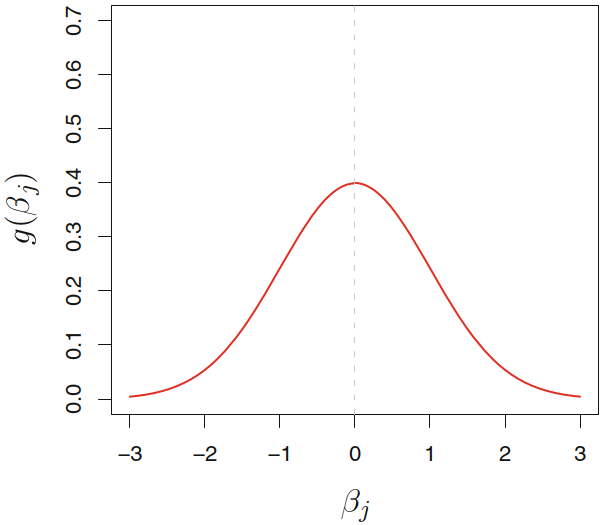
\includegraphics[width=7cm]{figure_6.11_1.png}
	\end{frame}
	
	\begin{frame}{Bayesian interpretation of ridge regression}
		\textit{Proof} \\
		The model underlying linear regression is $Y=X\beta+\epsilon$, where $\epsilon \sim \mathcal{N}(0, \sigma^2)$. In Bayesian statistics, $\beta$ is a random vector that has a prior distribution. We can get:
		\begin{align*}
			&\beta \sim \mathcal{N}(0, \frac{\sigma^2}{\lambda} I), \\
			&i.e., f_\beta(\beta)=(2\pi)^{-\frac{p}{2}}p^{-\frac{1}{2}}\exp(-\frac{1}{2}\beta^T\frac{\lambda}{\sigma^2}\beta)\\
			&Y|X,\beta \sim \mathcal{N}(X\beta, \sigma^2I), \\
			&i.e., f_{Y|X,\beta}(Y|X,\beta)=(2\pi)^{-\frac{n}{2}}n^{-\frac{1}{2}}\exp(-\frac{1}{2}(Y-X\beta)^T\frac{1}{\sigma^2}(Y-X\beta))
		\end{align*}
	\end{frame}
	
	\begin{frame}{Bayesian interpretation of ridge regression}
		The mode of posterior distribution (conditional distribution) of $\beta$ (assume $X$ is fixed):
		\begin{align*}
			& \hat{\beta}=\mathop{\arg\max}_{\beta} f_{\beta|X,Y}(\beta|X,Y)\\
			&=\mathop{\arg\max}_{\beta} \frac{f_{X,\beta}(X,\beta)f_{Y|X,\beta}(Y|X,\beta)}{f_{X,Y}(X,Y)} \\
			&=\mathop{\arg\max}_{\beta} \frac{f_X(X)f_{\beta|X}(\beta|X)f_{Y|X,\beta}(Y|X,\beta)}{f_{X,Y}(X,Y)} \\
			&=\mathop{\arg\max}_{\beta} f_\beta(\beta)f_{Y|X,\beta}(Y|X,\beta)
		\end{align*}
	\end{frame}
	
	\begin{frame}{Bayesian interpretation of ridge regression}
		\begin{align*}
			&=\mathop{\arg\max}_{\beta} \exp \big(-\frac{1}{2}\beta^T\frac{\lambda}{\sigma^2}\beta-\frac{1}{2}(Y-X\beta)^T\frac{1}{\sigma^2}(Y-X\beta)\big) \\
			&=\mathop{\arg\min}_{\beta} \frac{1}{2}\beta^T\frac{\lambda}{\sigma^2}\beta+\frac{1}{2}(Y-X\beta)^T\frac{1}{\sigma^2}(Y-X\beta) \\
			&=\mathop{\arg\min}_{\beta} (Y-X\beta)^T(Y-X\beta) + \lambda \beta^T\beta \\
			&=\mathop{\arg\min}_{\beta} \|X\beta-Y\|_2^2 + \lambda \|\beta\|_2^2
		\end{align*}
		\begin{proof}[\unskip\nopunct]\end{proof}
	\end{frame}
	
	\begin{frame}{Standardizing the predictors}
		For ordinary least squares, $X_j\hat{\beta}_j$ depends on the scaling of $X_j$. But for ridge regression, $X_j\hat{\beta}_{j,\lambda}$ will depend not only on the value of $\lambda$, but also on the scaling of the
		$j^{th}$ predictor. It may even depend on the scaling of other predictors. \\
		Standardize the predictors before ridge regression:
		\[
		\tilde{x_{ij}}=\frac{x_{ij}}{\sqrt{\frac{1}{n}\sum_{i=1}^{n}(x_{ij}-\overline{x}_j) ^2}}
		\]
	\end{frame}
	
	\begin{frame}{An application}
		Ridge regression more or less shrinks every dimension of the data by the same proportion. \\
		\vspace{0.5cm}
		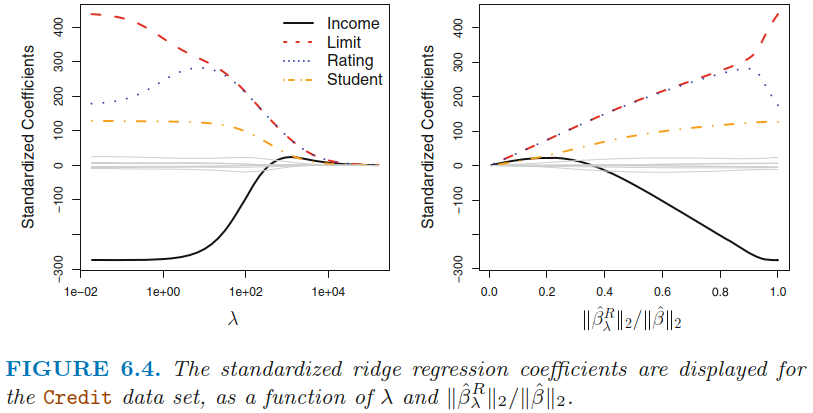
\includegraphics[width=10cm]{figure_6.4.png}
	\end{frame}
	
	\begin{frame}{An application}
		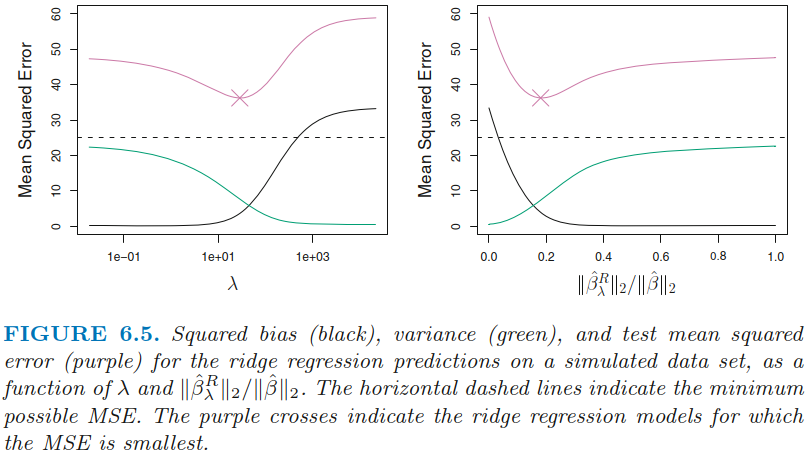
\includegraphics[width=10cm]{figure_6.5.png}
	\end{frame}
	
	\subsection{Lasso Regression}
	\begin{frame}{Lasso Regression}
		\[
		\hat{\beta}^R = \mathop{\arg\min}_{\beta} \sum_{i=1}^{n} (y_i-\beta_0-\sum_{j=1}^{p} \beta_jx_{ij})^2+\lambda\sum_{j=1}^{p}|\beta_j|
		\]
	\end{frame}
	
	\begin{frame}{Centered form}
		Transform the training data to centered form:
		\begin{align*}
			&X=[x_1-\overline{x},...,x_n-\overline{x}]^T \\
			&Y=[y_1-\overline{y}, ..., y_n-\overline{y}]^T \\
			&\beta=[\beta_1, ..., \beta_p]^T, \beta_0=\overline{y}-\beta^T\overline{x}
		\end{align*}
		Lasso Regression (centered):
		\begin{equation*}
			\hat{\beta}^L = \mathop{\arg\min}_{\beta} \|X\beta-Y\|_2^2 + \lambda \|\beta\|_1
		\end{equation*}
		Another formulation (centered):
		\begin{equation*}
			\hat{\beta}^L = \mathop{\arg\min}_{\beta} \|X\beta-Y\|_2^2,\ s.t.\ \|\beta\|_1 \leq t
		\end{equation*}
	\end{frame}
	
	\begin{frame}{Bayesian interpretation of lasso regression}
		Lasso regression is maximum a posteriori estimation (MAP) that assumes $\beta$ has prior distribution of $\beta \sim Laplace(0, \frac{2\sigma^2}{\lambda}I)$. \\
		\vspace{0.5cm}
		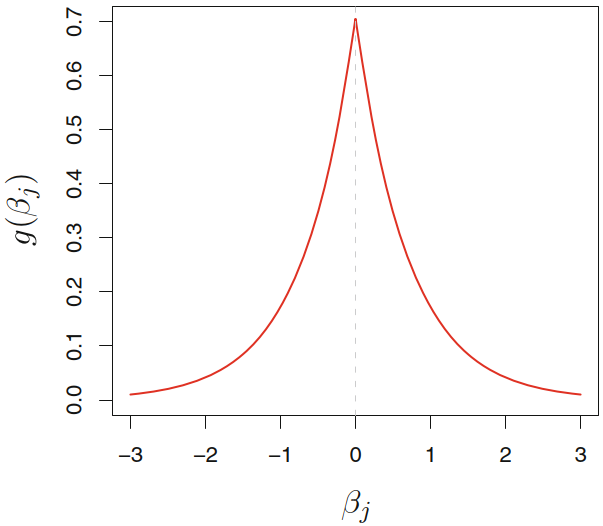
\includegraphics[width=7cm]{figure_6.11_2.png}
	\end{frame}
	
	\begin{frame}{Bayesian interpretation of lasso regression}
		\textit{Proof} \\
		The model underlying linear regression is $Y=X\beta+\epsilon$, where $\epsilon \sim \mathcal{N}(0, \sigma^2)$. In Bayesian statistics, $\beta$ is a random vector that has a prior distribution. We can get:
		\begin{align*}
			&\beta \sim Laplace(0, \frac{2\sigma^2}{\lambda} I), \\
			&i.e., f_\beta(\beta)=\frac{\lambda}{4\sigma^2}\exp(-\frac{\lambda\|\beta\|_1}{2\sigma^2})\\
			&Y|X,\beta \sim \mathcal{N}(X\beta, \sigma^2I), \\
			&i.e., f_{Y|X,\beta}(Y|X,\beta)=(2\pi)^{-\frac{n}{2}}n^{-\frac{1}{2}}\exp(-\frac{1}{2}(Y-X\beta)^T\frac{1}{\sigma^2}(Y-X\beta))
		\end{align*}
	\end{frame}
	
	\begin{frame}{Bayesian interpretation of lasso regression}
		The mode of posterior distribution (conditional distribution) of $\beta$ (assume $X$ is fixed):
		\begin{align*}
			& \hat{\beta}=\mathop{\arg\max}_{\beta} f_{\beta|X,Y}(\beta|X,Y)\\
			&=\mathop{\arg\max}_{\beta} \frac{f_{X,\beta}(X,\beta)f_{Y|X,\beta}(Y|X,\beta)}{f_{X,Y}(X,Y)} \\
			&=\mathop{\arg\max}_{\beta} \frac{f_X(X)f_{\beta|X}(\beta|X)f_{Y|X,\beta}(Y|X,\beta)}{f_{X,Y}(X,Y)} \\
			&=\mathop{\arg\max}_{\beta} f_\beta(\beta)f_{Y|X,\beta}(Y|X,\beta)
		\end{align*}
	\end{frame}
	
	\begin{frame}{Bayesian interpretation of lasso regression}
		\begin{align*}
			&=\mathop{\arg\max}_{\beta} \exp \big(-\frac{\lambda\|\beta\|_1}{2\sigma^2}-\frac{1}{2}(Y-X\beta)^T\frac{1}{\sigma^2}(Y-X\beta)\big) \\
			&=\mathop{\arg\min}_{\beta} \frac{\lambda\|\beta\|_1}{2\sigma^2}+\frac{1}{2}(Y-X\beta)^T\frac{1}{\sigma^2}(Y-X\beta) \\
			&=\mathop{\arg\min}_{\beta} (Y-X\beta)^T(Y-X\beta) + \lambda \|\beta\|_1 \\
			&=\mathop{\arg\min}_{\beta} \|X\beta-Y\|_2^2 + \lambda \|\beta\|_1
		\end{align*}
		\begin{proof}[\unskip\nopunct]\end{proof}
	\end{frame}
	
	\begin{frame}{An application}
		The lasso more or less shrinks all coefficients toward zero by a similar amount, and sufficiently small coefficients are shrunken all the way to zero. \\
		\vspace{0.5cm}
		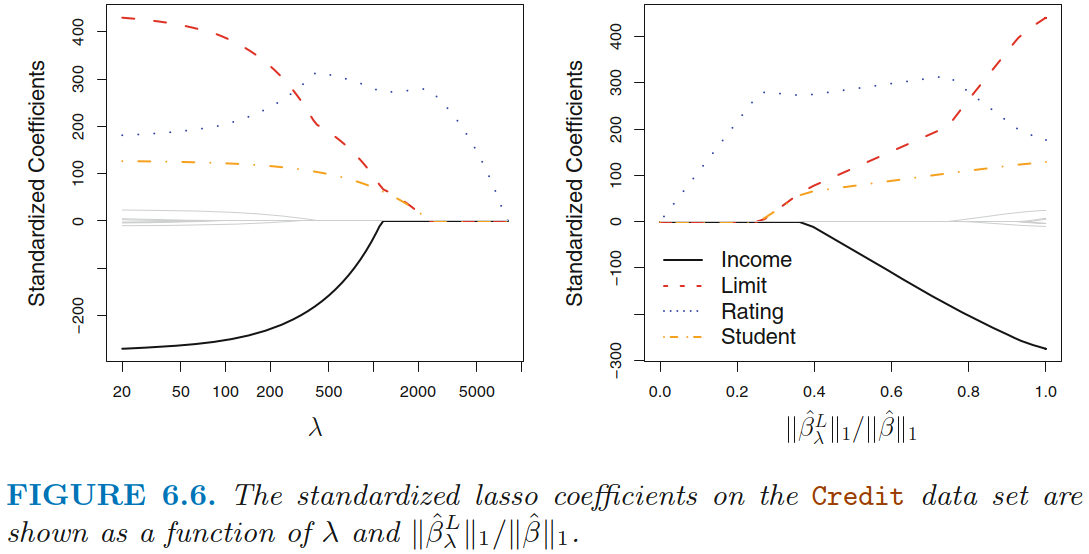
\includegraphics[width=10cm]{figure_6.6.png}
	\end{frame}
	
	\begin{frame}{Lasso estimates can shrink to 0 but ridge cannot }
		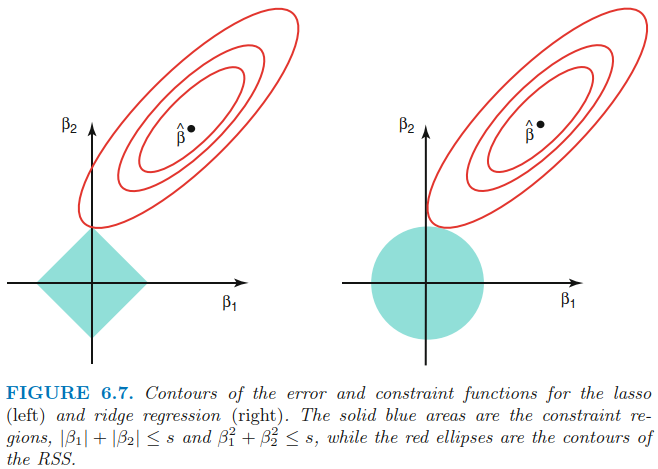
\includegraphics[width=10cm]{figure_6.7.png} \\
		\vspace{0.1cm}
		Reference \hyperlink{https://stats.stackexchange.com/questions/225319/is-there-a-mathematical-expression-that-shows-how-lasso-shrinks-coefficients-in}{\textit{link}} of proof.
	\end{frame}
	
	\begin{frame}{Comparison between Lasso and Ridge Regression}
		All 45 predictors were related to the response. \\
		\vspace{0.5cm}
		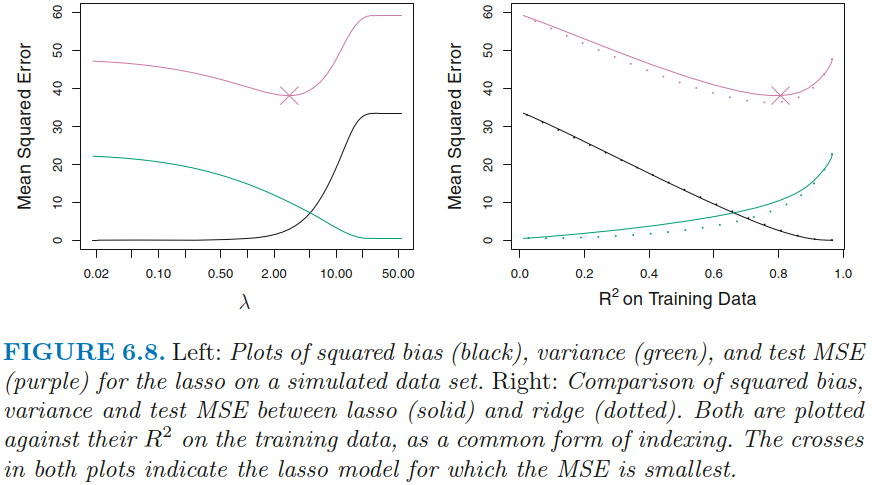
\includegraphics[width=10cm]{figure_6.8.png}
	\end{frame}
	
	\begin{frame}{Comparison between Lasso and Ridge Regression}
		Only two predictors are related to the response. \\
		\vspace{0.5cm}
		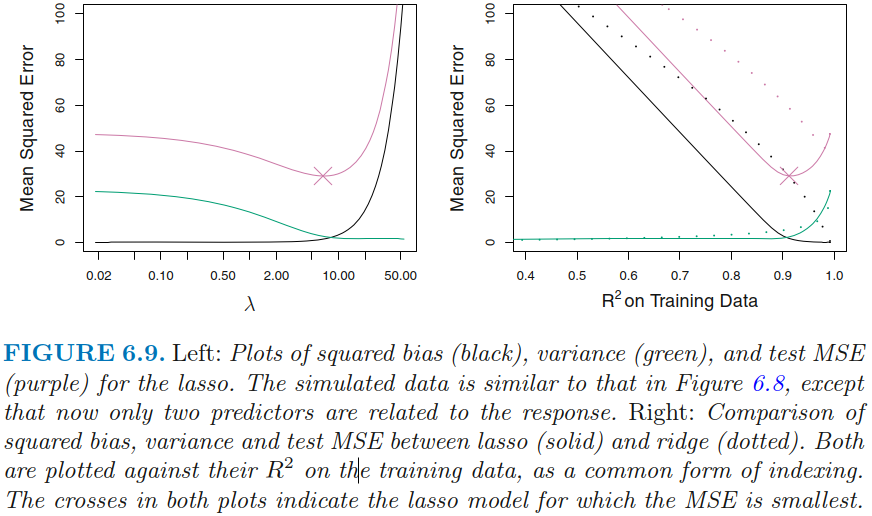
\includegraphics[width=10cm]{figure_6.9.png}
	\end{frame}
	
	\subsection{Parameter Selection}
	\begin{frame}{An example of cross-validation}
		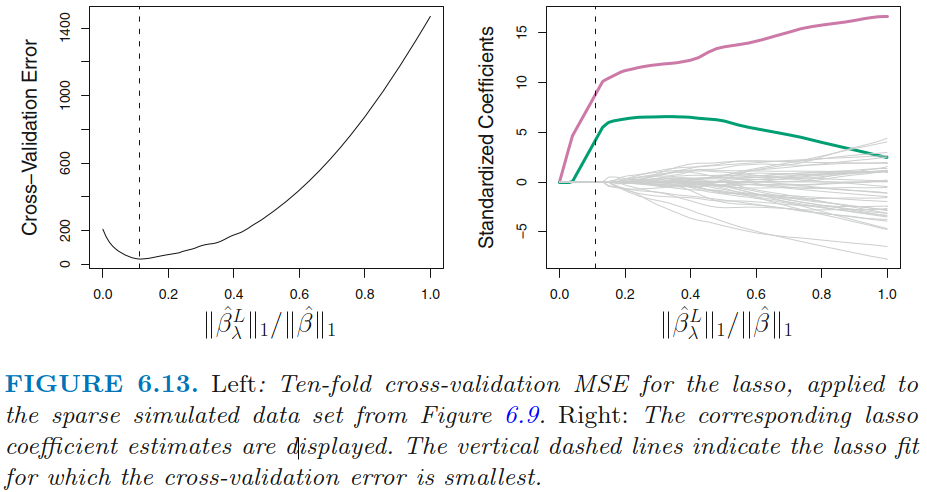
\includegraphics[width=10cm]{figure_6.13.png}
	\end{frame}

	\section{Dimension Reduction Methods}
	\begin{frame}{Outline}
		\tableofcontents[currentsection]
	\end{frame}
	
	\subsection{The Framework}
	\begin{frame}{The framework}
		Let $Z_1,Z_2,...Z_m$ represent $M<p$ linear combinations of original $p$ predictors. That is,
		\[
		Z_m=\sum_{j=1}^{p}\phi_{jm}X_j
		\]
		for some constants $\phi_{1m}, \phi_{2m},...,\phi_{pm}$. We can then fit the linear regression model
		\[
		y_i=\theta_0+\sum_{m=1}^{M}\theta_mz_{im}+\epsilon_i,\ \ i=1,2,...,n,
		\]
		using least squares.
	\end{frame}

	\subsection{Principle Components Regression}
	\begin{frame}{What is PCA?}
		\textbf{The target}: find the low-dimension representation of $X$ that explains the most variance of the covariance matrix of $X$. \\
		\textbf{The solution}: eigenvalue decomposition or singular value decomposition. \\
		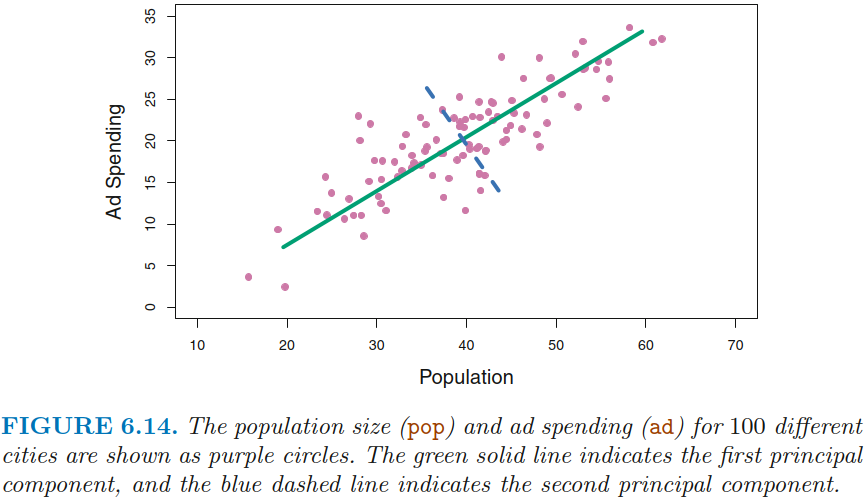
\includegraphics[width=10cm]{figure_6.14.png}
	\end{frame}
	
	\begin{frame}{Eigenvalues decomposition}
		\textit{Theorem}\\
		We can decompose any square, symmetric $n\times n$ matrix S as
		\[
		S=U\Lambda U^T=\sum_{i=1}^{n}\lambda_iu_iu_i^T,
		\]
		where $\Lambda=diag(\lambda_1,...,\lambda_n)$, with $\lambda_1\geq...\geq\lambda_n$ the eigenvalues. $U=[u_1,...,u_n]$ is a $n \times n$ orthonormal matrix ($U^TU=I$) that contains the eigenvectors.
	\end{frame}
	
	\begin{frame}{Variance maximization problem}
		Let data matrix $X=[x_1,...,x_n]\in \mathbb{R}^{p\times n}$, and assume $X$ is centered, which is $\hat{x}=\frac{1}{n}\sum_{i=1}^{n}x_i=0$. Then the sample covariance matrix is
		\[
		Var(X)=C=\frac{1}{n-1}XX^T.
		\]
		The projection of $X$ on a direction vector $u\ (\|u\|_2^2=1)$ can be represented as $uu^TX$, with $u^TX$ the transformed coordinates of $X$ on basis $u$. \\
		Then the \textbf{variance maximization problem} is
		\[
		\hat{u}=\mathop{\arg\max}_{u} Var(u^TX)=\mathop{\arg\max}_{u} u^TCu.
		\]
	\end{frame}
	
	\begin{frame}{Variance maximization problem}
		\textit{Solution} is $\hat{u}=u_1$, where $u_1$ is the first eigenvector of $C$.\\
		\vspace{0.5cm}
		\textit{Proof} \\
		Eigenvalue decomposition of $C$: 
		\[
		C=U\Lambda U^T.
		\] \\
		Let $v=U^Tu$, we have $\|v\|_2^2=v^Tv=u^TUU^Tu=u^Tu=1$,
		\begin{align*}
			&\max u^TCu = \max u^TU\Lambda U^Tu = \max v^T\Lambda v \\
			&=\max \lambda_1v_1^2 + ... + \lambda_pv_p^2,\ s.t. \|v\|_2^2=1.
		\end{align*}
		Because $\lambda_1 \geq...\geq\lambda_p$, we get $v^*=[1,0,...,0]^T$, and corresponding $u^*=Uv^*=[u_1,...,u_p]v^*=u_1$.
		\begin{proof}[\unskip\nopunct]\end{proof}
	\end{frame}
	
	\begin{frame}{An application of $u_1$}
		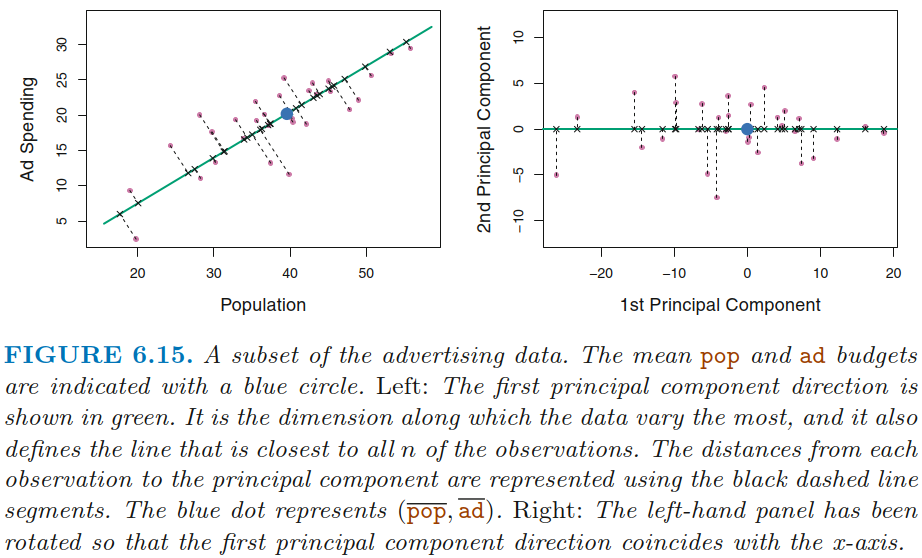
\includegraphics[width=10cm]{figure_6.15.png}
	\end{frame}
	
	\begin{frame}{Iteration method to find $k$ principle components}
		We say $u_1$ is the first principle component of $X$. The projection of $X$ on $u_1$ is $u_1u_1^TX$. The projection of $X$ on a hyperplane orthogonal to $u_1$ (deflation, the unexplained information by $u_1$) is
		\[
		X^{(2)}:=X-u_1u_1^TX=(I-u_1u_1^T)X.
		\]
		We get the second principle components by solving variance maximization problem on $X^{(2)}$:
		\begin{align*}
			&C^{(2)}=(I-u_1u_1^T)C(I-u_1u_1^T) \\
			&=(I-u_1u_1^T)\big(\sum_{i=1}^{n}\lambda_iu_iu_i^T\big)(I-u_1u_1^T) \\
			&=\sum_{i=2}^{n}\lambda_iu_uu_i^T.
		\end{align*}
	\end{frame}
	
	\begin{frame}{Iteration method to find $k$ principle components}
		\[
		C^{(2)}=\sum_{i=2}^{n}\lambda_iu_uu_i^T
		\]
		\begin{itemize}
			\item The largest eigenvalue of $C^{(2)}$ is $\lambda_2$.
			\item The second principle component is $u_2$.
		\end{itemize}
		After $k$ iterations, we get the $k$ directions (principle components) of largest variance, which is
		\[
		U^{(k)}=[u_1,u_2,...,u_k].
		\]
		Then the k-dimension representation of $X$ is
		$
		U^{(k)T}X,
		$
		and the rank-k approximation of $X$ is
		\[
		U^{(k)}U^{(k)T}X.
		\]
	\end{frame}
	
	\begin{frame}{Theorems of PCA}
		\textit{Theorem} $\hat{X}^{(k)}=U^{(k)}U^{(k)T}X$ solves the problem
		\[
		\mathop{\arg\min}_{\hat{X}^{(k)}} \|\hat{X}^{(k)}-X\|_F,\ s.t. Rank(\hat{X}^{(k)})\leq k,
		\]
		and we have
		\begin{align*}
			&\frac{1}{n-1}\|\hat{X}^{(k)}-X\|_F^2=\frac{1}{n-1}\|U^{(k)}U^{(k)T}X-X\|_F^2\\
			&=\frac{1}{n-1}\|(I-U^{(k)}U^{(k)T})X\|_F^2 \\
			&=Trace((I-U^{(k)}U^{(k)T})C(I-U^{(k)}U^{(k)T})) \\
			&=\lambda_{k+1} + ... + \lambda_p.
		\end{align*}
	\end{frame}
	
	\begin{frame}{Principle components regression and an example}
		Settings in PCR replace $X$ with $U^{(k)T}X$. \\
		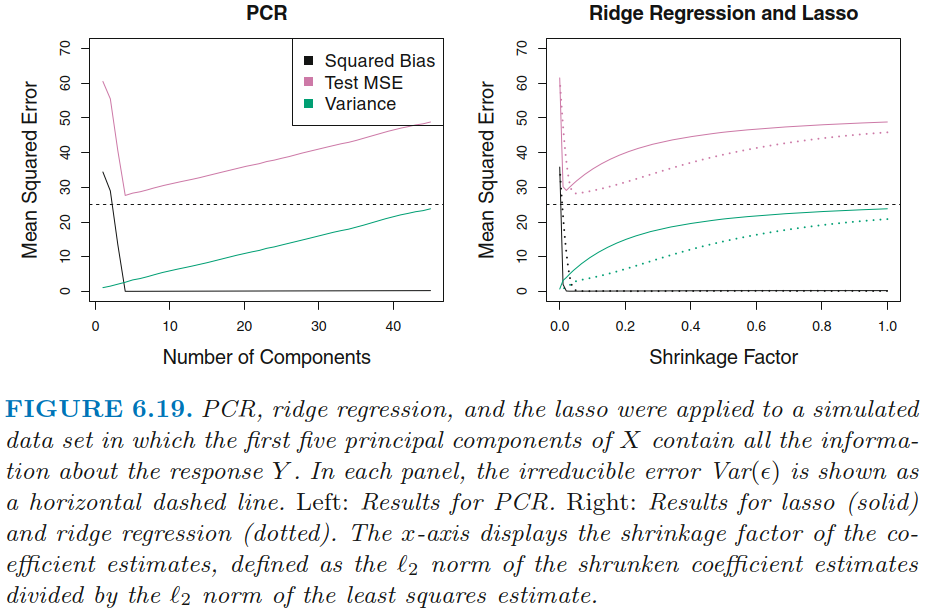
\includegraphics[width=10cm]{figure_6.19.png}
	\end{frame}
	
	\subsection{Partial Least Squares}
	\begin{frame}{Partial Least Squares}
		Partial least squares (PLS) is a supervised alternative to PCR.
		\begin{itemize}
			\item PLS computes the first direction $Z_1$ by setting each $\phi_{j1}$ equal to the coefficient from the simple linear regression of $Y$ onto $X_j$.
			\item PLS then projects $X$ on a hyperplane orthogonal to $Z_1$, which can be interpreted as the remaining information that has not been explained by the first PLS direction.
			\item PLS computes the second direction $Z_2$ using this orthogonalized data in exactly the same fashion as $Z_1$ was computed based on the original data.
			\item Iterate.
		\end{itemize}
		In practice it often performs no better than ridge regression or PCR (reduce bias but also increase variance).
	\end{frame}

	\section{Considerations in High Dimensions}
	\begin{frame}{Outline}
		\tableofcontents[currentsection]
	\end{frame}
	\begin{frame}{Curse of dimension}
		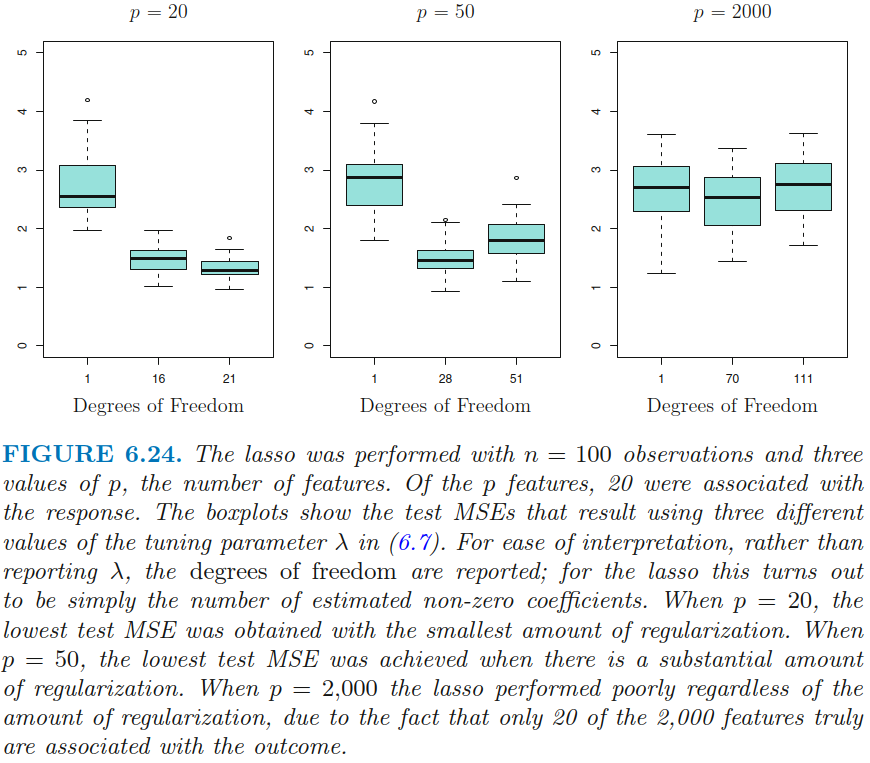
\includegraphics[width=9cm]{figure_6.24.png}
	\end{frame}
	\begin{frame}{Considerations}
		\begin{itemize}
			\item Adding noise features that are not truly associated with the response will lead to a deterioration in the model.
			\item In the high-dimensional setting, the multicollinearity problem is extreme. The model we have identified is simply one of many possible models for predicting, and it must be validated on independent data sets.
		\end{itemize}
	\end{frame}
\end{document}
